\documentclass{article}
\usepackage{amsthm}
\usepackage{amsmath}
\usepackage{graphicx}
\usepackage{tikz}
\usepackage{wasysym}

\newtheorem{problem}{Problem}

\begin{document}
\title{Graphs}
\author{Henry Z. Lo}
\maketitle

\section{Graphs}
\subsection{Definition}
Graphs are a combination of \textit{vertices} (or nodes) and \textit{edges}.  Edges connect vertices.  See an example in Figure \ref{graph-example}.

\begin{figure}
\centering
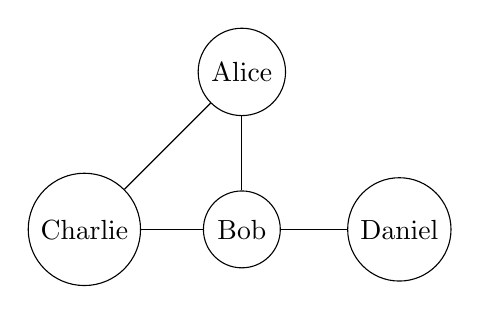
\begin{tikzpicture}[node distance=2cm, main node/.style={draw,circle}]
\node[main node]             (a) {Alice};
\node[main node, below of=a] (b) {Bob};
\node[main node, left of=b]  (c) {Charlie};
\node[main node, right of=b]  (d) {Daniel};
\path
(a) edge node {} (b)
    edge node {} (c)
(b) edge node {} (d)
    edge node {} (c);
\end{tikzpicture}
\caption{Example of a graph representing friendships. \label{graph-example}}
\end{figure}

Graphs can have \textit{directed} or \textit{undirected} edges.  Figure \ref{graph-example} shows an undirected graph.  Edges here represent symmetric friendships, and so do not need to have direction.  Figure \ref{directed-graph} shows the water cycle in a directed graph.  Here, directed edges makes sense because water does not evaporate and then become groundwater.

\begin{figure}
\centering
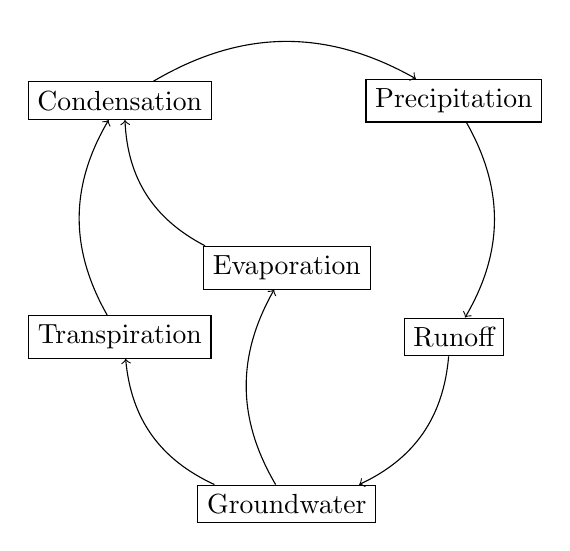
\begin{tikzpicture}[->, node distance=3cm, main node/.style={draw}]
\node[main node]             (p) {Precipitation};
\node[main node, below of=p] (r) {Runoff};
\node[main node, below left of=r]  (g) {Groundwater};
\node[main node, above left of=g]  (t) {Transpiration};
\node[main node, above of=g]  (e) {Evaporation};
\node[main node, above of=t]  (c) {Condensation};

\path
(p) [bend left] edge node {} (r)
(r) edge node {} (g)
(g) edge node {} (t)
    edge node {} (e)
(t) edge node {} (c)
(c) edge node {} (p)
(e)  edge node {} (c);
\end{tikzpicture}
\caption{Directed graph representing the water cycle. \label{directed-graph}}
\end{figure}

We can define the following on a graph:
\begin{itemize}
\item \textbf{Path}: a path between two nodes is a sequence of edges connecting them.
\item \textbf{Cycle}: a path which begins and ends at the same vertex.
\item \textbf{Connected component}: a set of nodes which have paths to each other.
\end{itemize}

\begin{figure}
\centering
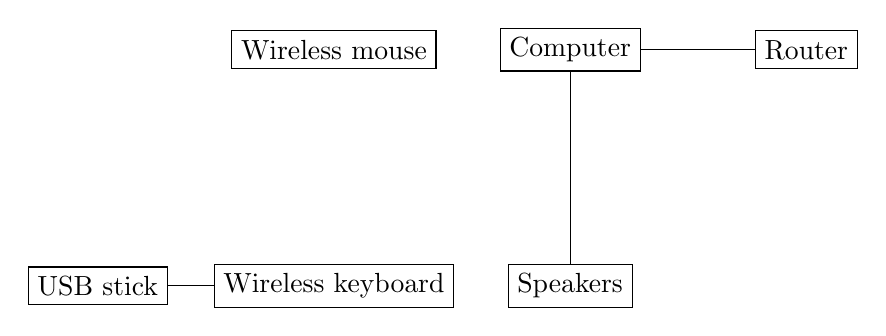
\begin{tikzpicture}[node distance=3cm, main node/.style={draw}]
\node[main node]             (a) {Wireless mouse};
\node[main node, below of=a] (b) {Wireless keyboard};
\node[main node, right of=a]  (c) {Computer};
\node[main node, right of=b]  (d) {Speakers};
\node[main node, right of=c]  (e) {Router};
\node[main node, left of=b] (f) {USB stick};
\path
(c) edge node {} (d)
    edge node {} (e)
(b) edge node {} (f);
\end{tikzpicture}
\caption{Example of a graph with three connected components. \label{graph-example}}
\end{figure}

Edges can have (and often do) weights, or numerical values assigned to  them.  They can represent anything from strength of friendship, time it takes on a road, etc.

\subsection{Relationship with trees}
A tree is a type of graph which has the following properties:
\begin{itemize}
\item It has one connected component.
\item It does not have cycles with more than 2 nodes.
\item We select some node as a root.
\end{itemize}

Because of this, we can define a \textit{spanning tree} on a graph, which contains the same number of nodes, but with no cycles.  This type of structure can be organized into a tree.  There are many \textit{spanning trees} for a graph.

\section{Representations}

Graphs can be represented in multiple ways using code, each with different performance trade-offs.  We discuss several common representations, analyze their performance, and demonstrate their use on the graph in figure \ref{graph}.

\begin{figure}
\centering
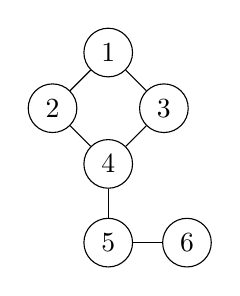
\begin{tikzpicture}[main node/.style={draw, circle}]
\node[main node]             (1) {1};
\node[main node, below left of=1] (2) {2};
\node[main node, below right of=1] (3) {3};
\node[main node, below right of=2] (4) {4};
\node[main node, below of=4] (5) {5};
\node[main node, right of=5]  (6) {6};
\path
(1) edge node {} (2)
    edge node {} (3)
(4) edge node {} (2)
    edge node {} (3)
    edge node {} (5)
(6) edge node {} (5);
\end{tikzpicture}
\caption{Example of an undirected, unweighted graph. \label{graph}}
\end{figure}

\subsection{Object representation}
Representing the graph as a set of edges and a set of vertices is natural in object-oriented languages.  In this approach, we get a \texttt{Set<Node> nodes} and \texttt{Set<Edge> edges}.  We assume \texttt{Edge} to contain two \texttt{Node}s, though it may also contain direction and weight if needed.

Representing the graph in figure \ref{graph} with these objects, we get:
\begin{verbatim}
Set<Node> nodes == {1,2,3,4,5,6}
Set<Edges> edges == {(1,2),(1,3),(2,4),(3,4),(4,5),(5,6)}
\end{verbatim}

For performance analysis, we assume that both the set of nodes and set of edges are hashsets, though treesets may be more appropriate when we want to keep edge lists sorted.

Whether \texttt{edges} should contain two copies of each edge, e.g. (1,2) and (2,1), depends on if the two are considered distinct.

\subsection{Adjacency matrix}
A very different representation consists of a $|V|\times |V|$ matrix:

\begin{center}
\begin{tabular}{c|cccccc}
& 1 & 2 & 3 & 4 & 5 & 6 \\
\hline
1 & 0 & 1 & 1 & 0 & 0 & 0 \\
2 & 1 & 0 & 0 & 1 & 0 & 0 \\
3 & 1 & 0 & 0 & 1 & 0 & 0 \\
4 & 0 & 1 & 1 & 0 & 1 & 0 \\
5 & 0 & 0 & 0 & 1 & 0 & 1 \\
6 & 0 & 0 & 0 & 0 & 1 & 0 \\
\end{tabular}
\end{center}
In this matrix, each both rows and columns represent nodes.  A cell $x_{ij}$ in the matrix has a 1 if an edge exists between node $i$ and node $j$, and 0 otherwise.

If the graph has edge weights, these weights go in the cell in place of the 1.  This assumes that an edge weight of 0 implies no edge.

The typical scheme to handle directed edges makes $x_{ij}$ positive if an edge goes from node $i$ to node $j$, and negative vice versa.

\subsection{Adjacency list}
An adjacency list consists of a hash table.  Each node is a key, and a node maps to a list of nodes that the key shares an edge with.

For the graph in figure \ref{graph}, we get:
\begin{center}
\begin{tabular}{c|l}
key & value \\
\hline
1 & $2 \rightarrow 3$ \\
2 & $4 \rightarrow 1$ \\
3 & $4 \rightarrow 1$ \\
4 & $2 \rightarrow 3 \rightarrow 5$ \\
5 & $6 \rightarrow 4$ \\
6 & 5 \\
\end{tabular}
\end{center}

Like the adjacency matrix, this representation does not use an explicit edge object.  For weighted graphs, values will be lists of weight / node tuples.  For directed graphs, key nodes will be source nodes, and value nodes will be destination nodes.

\subsection{Efficiency comparison}

\begin{center}
\begin{tabular}{l|ccc}
 & Object & Matrix & List \\
\hline
Storage & $O(V+E)$ & $O(V^2)$ & $O(V+E)$ \\
Add vertex & $O(1)$ & $O(V^2)$ & $O(1)$ \\
Remove vertex & $O(E)$ & $O(V^2)$ & $O(E)$ \\
Add edge & $O(1)$ & $O(1)$ & $O(1)$ \\
Remove edge & $O(1)$ & $O(1)$ & $O(V)$ \\
All edges from $V$ & $O(E)$ & $O(V)$ & $O(1)$ 
\end{tabular}
\end{center}

\section{Minimum Spanning Trees}
Suppose you are a telecom company, and you need to lay cable.  You need to hit each home (node), but taking different paths may result in different costs, e.g. you may need to dig deeper in some areas.

\subsection{Prim's algorithm}
Prim's greedy method:
\begin{enumerate}
\item Keep track of \texttt{visited}, a set of vertices in the spanning tree we are building.
\item Put any vertex into \texttt{visited}.
\item Find the lowest weighted edge that connects a node in \texttt{visited} with a node not in \texttt{visited}.
\item Add that vertex to \texttt{visited}.
\item Repeat from step 2 until all nodes are visited.
\end{enumerate}

The algorithm operates on every vertex once.  We can assume that \texttt{visited} is a hash set.  What is the runtime then of step 3?  In the object representation and list representations, it is $O(E)$, but note that if we keep the edge to vertices sorted, we can grab the lowest weighted edge in $O(\log E)$.

The algorithm then becomes:
\begin{enumerate}
\item Keep track of \texttt{visited}, a set of vertices in the spanning tree we are building, and \texttt{h}, a heap sorted by edge weight.
\item Put any vertex into \texttt{visited}.
\item For each neighbor vertex not in \texttt{visited}, add the connecting edge to \texttt{h}.  If the vertex already exists, replace the edge in \texttt{h} if the new edge has a lower weight.
\item Get the vertex with the lowest edge weight in \texttt{h} , an add that vertex to \texttt{visited}.
\item Repeat from step 2 until all nodes are visited.
\end{enumerate}

The runtime for this algorithm is $O(V\log E)$.

The greedy choice in this method picks the lowest weighted valid edge to add to our tree.  Note that this greedy edge joins two sets of nodes.  In our MST, we only need one edge to join these sets, and if we choose anything other than the least weighted edge, we end up with a greater total edge sum.

\subsection{Kruskal's algorithm}
Kruskal's algorithm is another greedy method:
\begin{enumerate}
\item Separate each node into its own set.
\item Pick the lowest weighted edge which connects two sets.
\item Store this edge, and merge the two sets.
\item Repeat from step 2 until all nodes are in the same set.
\end{enumerate}

As with Prim's algorithm, sorting helps.  After step 1, we can insert a step to sort the edges first.  The set merging operation can be done in $O(\log V)$ time using union-finds, but this will not be discussed.

The runtime for this algorithm is $O(E\log V)$.

\end{document}